\section{Internal Combustion Engine Simulator}
%
ICESym es un simulador de motores de combustión interna que  utiliza modelos 0D
para la cámara de combustión y 1D para el flujo a través del sistema de
intercambio de gases.
%
Esta combinación permite evaluar la \emph{performance} de un motor a un costo
computacional bajo; además la implementación de entrada y salida de datos
permite utilizar el simulador como una \emph{caja negra}.
%
Esto permitió incluir al simulador en un \emph{script} como una función a la que
se le otorga un conjunto de parámetros de entrada y devuelve los resultados de
la simulación en un formato que permite la lectura y evaluación de los mismos.
%
Contiene en su código las rutinas necesarias para simular el ciclo operativo y la
geometría del MRCVC.

Se realizaron modificaciones menores al simulador para facilitar la ejecución en
conjunto con el optimizador, algunas de estas modificaciones fueron:
%
\begin{enumerate}
    \item Modificar el formato de los archivos de salida, eliminando valores que
no se utilizaron, con el fin de reducir el tamaño de los archivos de salida,
facilitar la lectura y el procesamiento de datos.
    \item Incluir una opción para elegir entre un modelo de $C_D$ de una o dos
variables.
    \item Modificar el área de referencia.
    \item Agregar una interpolación bilineal para poder trabajar con el mapa de
$C_D$.
\end{enumerate}


\section{Modificaciones a ICESym}
%%%%%%%%%%%%%%%%%%%%%%%%%%%%%%%%%%%%%%%%%%%%%%%%%%%%%%%%%%%%%%%%%%%%%%%%%%%%%%%
\subsection{Flujo a Través de los Puertos}
%
Se introdujo una opción para poder ejecutar ICESym con un modelo del coeficiente
de descarga que dependa de dos variables, diferencia de presión y \emph{alzada}
o apertura del puerto $C_D = f(lv; \Delta P)$.
%
Esto significó agregar un \emph{switch} en el código que permita seleccionar
entre un modelo de una o dos variables, con el agregado de las instrucciones de
lectura de datos y armado de un arreglo bidimensional que contiene los valores
del mapa de $C_{D}$ en un orden dado.
%
Con esto se construye un mapa del coeficiente de descarga de la forma $C_D =
f(lv, dp)$, que se utiliza para calcular el área efectivo del puerto.


\nomenclature[F]{\(\Delta P\)}{Diferencia de presión a través de un puerto}


Independientemente de la cantidad de variables que formen parte del $C_{D}$, a
ICESym se introduce un vector o matriz para el caso 1D o 2D respectivamente.
%
En ambos casos se intrudce una cantidad discreta de valores por lo que es
necesario realizar una interpolación lineal o bilineal para utilizar el valor de
$C_{D}$.
%
La interpolación lineal 1D es parte del código de ICESym, mientras que la
interpolación 2D o bilineal se introdujo como parte de este trabajo.

Esta última se realiza sobre una malla rectangular, de modo de reutilizar el
código existente para el caso 1D y realizar  simplemente una interpolación
lineal entre dos valores en planos con datos conocidos.

% En el algoritmo~\ref{algo:interpolacion_lineal} se describe la interpolación 1D
% comentada del código de ICESym.
%
Para el caso bidimensional, se utiliza la interpolación lineal 1D entre
interpolar entre los planos correspondientes a los valores requeridos, ver
Figura~\ref{fig:interp_bilineal}.

\begin{figure}
    \centering
    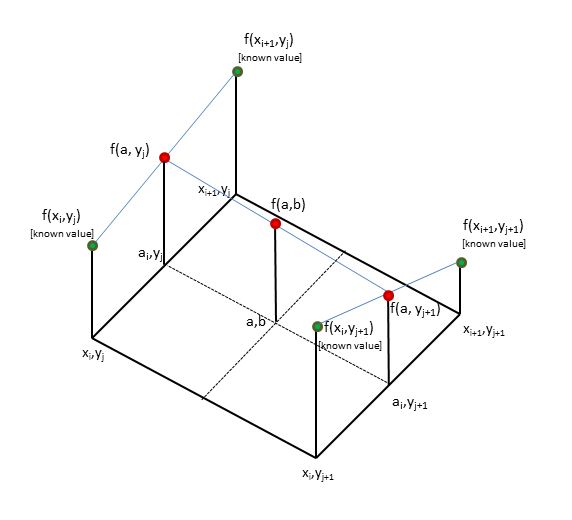
\includegraphics[width=0.7\textwidth]{interpolacion_bilineal.png}
    %
    \caption{Interpolación bilineal\protect\footnotemark}\label{fig:interp_bilineal}
    % \footnote{A}}
\end{figure}

\footnotetext{\url{https://stackoverflow.com/questions/8808996/bilinear-interpolation-to-enlarge-bitmap-images}}

Si bien hay otros métodos de interpolación para estimar el valor de $C_D$ a
partir de una nube de puntos, este método es sencillo y da resultados
satisfactorios.
%
En la Figura~\ref{fig:bilineal} se muestra un ejemplo del error obtenido con
este método para interpolar una función de prueba $f=\sin\left(\sqrt(x^2 + y^2)\right)$.

\begin{figure}
    \centering
    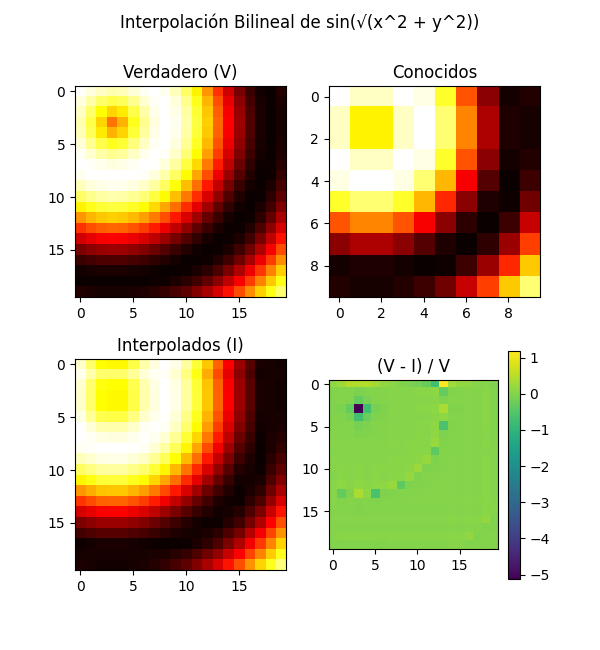
\includegraphics[width=0.7\textwidth]{bilineal.png}
    \caption{Interpolación bilineal de $\sin(\sqrt(x^2 + y^2))$}\label{fig:bilineal}
\end{figure}

La malla rectangular requerida para la interpolación bilineal del mapa de
$C_{D}$ se realizará a partir de los valores conocidos de $C_D$ resultantes de
las flujometrías con \emph{OpenFOAM}~\parencite{openfoam}.
%
Debido al costo computacional que requieren las flujometrías, solo una cantidad
reducida de puntos se obtendrá con este método, lo cual significa que se tiene
como punto de partida una malla no rectangular, por lo que se utiliza un método
intermedio para obtener una matriz de puntos que pueda ser leída por la
interpolación bilineal.

Se probaron dos métodos para realizar la interpolación, el método del punto más
cercano (MC) y la interpolación por la suma de la inversa de la distancia o IDW por
sus siglas en inglés (\emph{Inverse Distance Weighting}).
%
Estos se combinan con métodos de suavizado de promedio móvil con los $n$ valores
más cercanos.

El método del punto más cercano consiste en asignar para cada par $(x, y)$ el
valor conocido más cercano, el algoritmo se indica en el
algoritmo~\ref{algo:mas_cercano}.

\begin{algorithm}
 \caption{Interpolación por punto más cercano}\label{algo:mas_cercano}
    \KwIn{\\
        $V_x, V_y$: valores de $x, y$ en los que se conoce el valor en $z$.\\
        $V_z$: valores conocidos de $z$.\\
        $I_x$: $n$ puntos de $x$ donde se quiere interpolar\\
        $I_y$: $m$ puntos de $y$ donde se quiere interpolar\\
        }

    \KwResult{Devuelve una matriz $I_{[n,m]}$ con los valores interpolados,
      donde a cada punto $I(x,y)$ se le asigna al valor de $V_z$ más cercano
      conocido. Da como resultado superficies escalonadas.}

    \BlankLine
     $I=zeros_{[n,m]}$\;
     \For{$i \gets 0$\KwTo$n$}{
        \For{$j \gets 0$\KwTo$m$}{
          $d = \sqrt{{(V_x - I_{xi})}^2 + {(V_y - I_{yj})}^2}$\;
            $I[i,j] = v_z[\min(d)]$\;
        }
     }
\end{algorithm}

La interpolación IDW consiste en asignar a cada punto el resultado de un
promedio de los valores cercanos al punto en cuestión, ponderado por la
distancia elevado a un exponente arbitrario $p$.
%
Cuanto más grande el valor de $p$, más sensible es el método a los valores
cercanos.
%
La formulación de este método se ve en la ecuación~(\ref{eq:idw}) y el
algoritmo~\ref{algo:IDW}.
%
En la Figura~\ref{fig:mapas_interpolados} se muestra una comparación de ambos
métodos, para una malla de $C_{D}=f(\Delta_{P}, l_{v})$ generada al azar.

\begin{equation} \label{eq:idw}
    f_p = \frac{\sum_{i=1}^{n} \frac{z_i}{d_i^p}} {\sum_{i=1}^{n}
    \frac{1}{d_i^p}}
\end{equation}

\begin{algorithm}
    \caption{Interpolación IDW}\label{algo:IDW}
    \KwIn{\\
        $V_x, V_y$: valores de $x, y$ en los que se conoce el valor en $z$.\\
        $V_z$: valores conocidos de $z$.\\
        $I_x$: $n$ puntos de $x$ donde se quiere interpolar\\
        $I_y$: $m$ puntos de $y$ donde se quiere interpolar\\
        $p$: potencia a la que se eleva cada peso\\
        }

    \KwResult{Interpolación ponderada por inverso de la distancia. Dependiendo
      del valor de $p$, se obtienen valores más o menos suavizados.}

    \BlankLine
    $I=zeros_{[n,m]}$\;
    \For{$i \gets 0$\KwTo$n$}{
        \For{$j$\gets 0 \KwTo$m$}{
          $d = {\left[{(V_x - I_{xi})}^2 +{(V_y - I_{yj})}^2\right]}^{\frac{p}{2}}$\;
          \eIf{$\exists i : d[i] = 0$}{
            $I[i, j] = V_z[i]$\;
          }{
            $I[i,j] = \frac{\sum{V_{zi}/d_i}}{\sum \frac{1}{d}}$\;
          }
        }
     }
\end{algorithm}

\begin{figure}
    \centering
    \begin{subfigure}{0.4\textwidth}
        \centering
        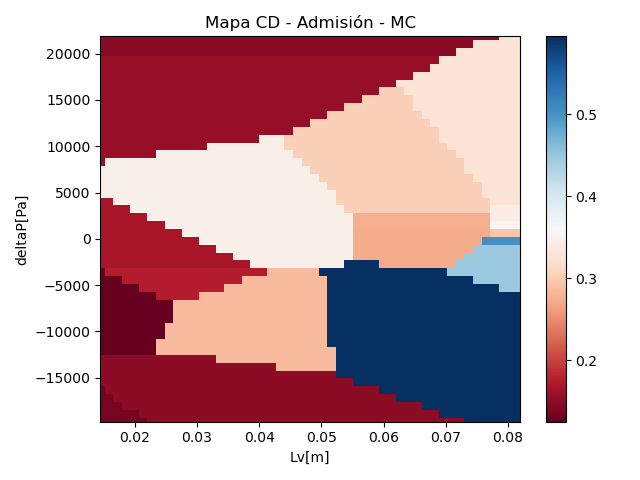
\includegraphics[width=\textwidth]{mapa_cd/mc_mapa_adm.png}
        \caption{Punto Más Cercano sin suavizar}
    \end{subfigure}
    \hfill
    \begin{subfigure}{0.4\textwidth}
        \centering
        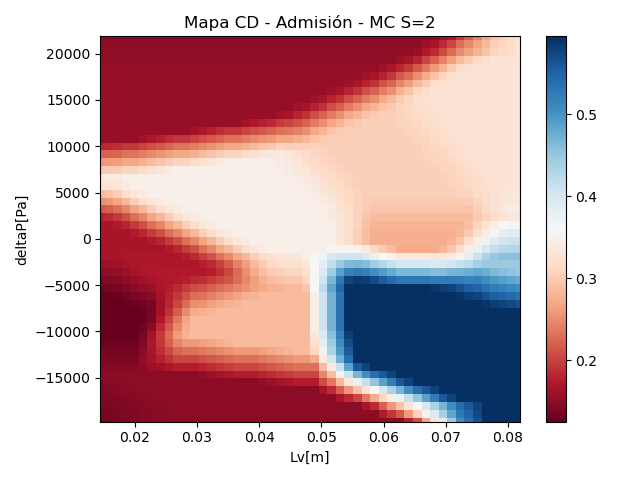
\includegraphics[width=\textwidth]{mapa_cd/mc_s2_mapa_adm.png}
        \caption{Más Cercano ($S=2$)}
    \end{subfigure}
    \hfill
    \begin{subfigure}{0.4\textwidth}
        \centering
        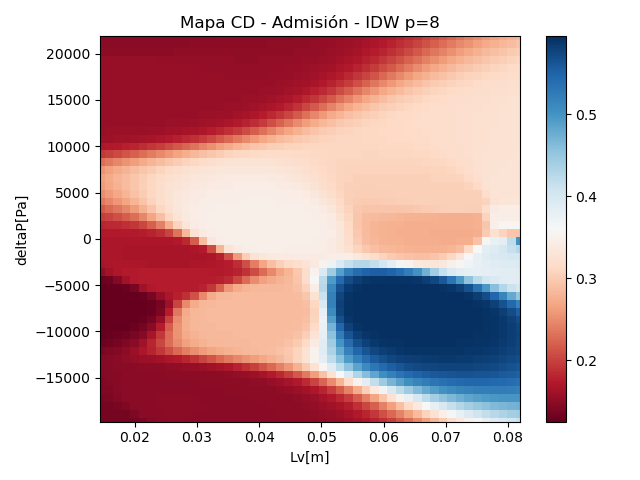
\includegraphics[width=\textwidth]{mapa_cd/idw8_mapa_adm.png}
        \caption{IDW ($p=8$)}
    \end{subfigure}
    \hfill
    \begin{subfigure}{0.4\textwidth}
        \centering
        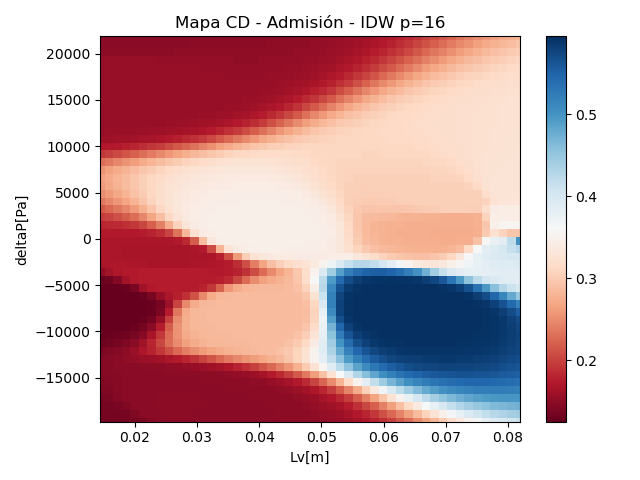
\includegraphics[width=\textwidth]{mapa_cd/idw16_mapa_adm.png}
        \caption{IDW ($p=16$)}
    \end{subfigure}
    \caption{Comparación de interpolaciones}\label{fig:mapas_interpolados}
\end{figure}

%%%%%%%%%%%%%%%%%%%%%%%%%%%%%%%%%%%%%%%%%%%%%%%%%%%%%%%%%%%%%%%%%%%%%%%%%%%%%%%

\subsection{Área de Referencia}
%
El área de referencia utilizada por ICESym es el área de
cortina~(\ref{eq:area_cortina}) y se expresa en el código del programa como el
área efectiva $F_{V}=A_{R}\cdot C_{D}$.
%
Como se indicó en el apartado~\ref{sec:cap2_cd}, para el  MRCVC el área de
referencia es el área frontal del puerto expuesta a la cámara, calculada como la
altura de la ranura $h_{p}$ multiplicada por la distancia entre el borde del
puerto y la paleta que delimita la cámara, denominada como $l_{v}$.

%
% En la Figura~\ref{fig:area_referencia} se ilustran las áreas de referencia para
% una posición del rotor en la que hay solape de cámaras con $\theta = 55^\circ$.
%
Este valor se afecta por el coeficiente de descarga intermedio $C_{D,int}$, que
puede ser un valor fijo o el resultado de interpolar de un mapa de $C_D$ para un
valor de cuerda y $\Delta_P$ dado, como se indica en la ecuación~(\ref{eq:fv}).

\begin{equation}\label{eq:fv}
    F_v = C_{D,int}\cdot h_{p}\cdot l_{v} = 0,0294\cdot C_{D,int}\cdot l_{v}
\end{equation}

% \begin{figure}
%     \centering
%     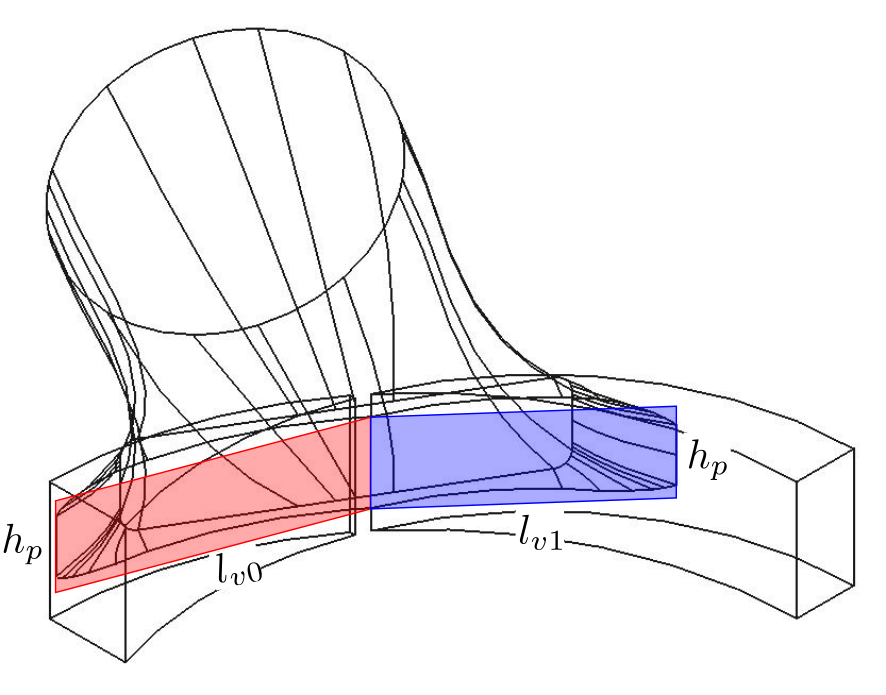
\includegraphics[]{area_referencia.png}
%     \caption{Área de referencia}\label{fig:area_referencia}
% \end{figure}

Tanto al inicio como al cierre del puerto ocurre solape de cámaras, por lo que
en estos intervalos angulares hay un valor de $C_D$ para cada cámara.
%
Este se calcula con el flujo másico que atraviesa los parches correspondientes
a cada cámara y el área de puerto expuesta por cada cámara.
% TODO: ver nota 8

\subsection{Interfaz con Optimizador}
%
Para lograr ejecutar el simulador automáticamente, se creó una librería de
funciones capaz de tomar como dato de entrada un archivo de configuración que
incluye geometría, velocidades a ejecutar y cantidad de ciclos de simulación
entre otros.

Para ejecutar una instancia de ICESym se puede utilizar la interfaz gráfica de
usuario (GUI) ó ejecutarlo por línea de comando desde una consola.
%
La simulación se realiza de manera automática aprovechando la cualidad de ``caja
negra'' de ICESym y se utiliza la interfaz de línea de comandos.
%
El simulador de motores se ejecuta como un archivo de Python ``>> python
main.py'', este archivo contiene las instrucciones que lanzan la simulación del
motor con una configuración dada.
%

ICESym requiere de un archivo de configuración con los datos de la simulación a
realizar, se organizan como:

\begin{forest}
  [config.py
    [Atmoshperes]
    [Junctions]
    [Simulator]
    [Cylinders
      [Combustion]
      [Fuel]
      [Inyection]
      [Valves]]
    [Tanks]
    [Tubes]
  ]
\end{forest}

\begin{itemize}
  \item Atmoshperes: contiene la presión, densidad y velocidad de la atmósfera,
condición de contorno de la simulación
  \item Cylinders: geometría y condiciones de contorno, estado inicial,
combustible, como así también de las válvulas.
  \item Valves: geometría, tipo de válvula, modelo de $C_{D}$, perfil de alzada y
datos de $C_{D}$, tubo y conectado.
  \item Junctions: contiene información de las uniones entre elementos (tubos,
tanques, cilindros y atmósfera)
  \item Simulator: configuración de la simulación, velocidades a simular,
propiedades de gas, combustible, directorios y demás
  \item Tanks: volumen, masa y temperatura de pared de tanques
  \item Tubes: geometría, cantidad de nodos y conexiones
\end{itemize}

Los elementos de configuración intervenidos son Cylinders, Valves y Simulator;
donde se pueden modificar según necesidad los siguientes valores:

\begin{itemize}
  \item Simulator:
        \begin{itemize}
          \item RPMS: Velocidades a simular (por ejemplo una lista de [1000; 2000; \ldots 9000)
          \item NCYCLES: cantidad de ciclos por velocidad (un entero mayor o igual a 1)
          \item FOLDER NAME: nombre de la carpeta donde se guardan los
resultados de la simulación
          \item SHOW INFO: selector para mostrar o no información (0: no, 1:sí)
          \item CONFIG DATA: archivo donde se guardan los datos de configuración
        \end{itemize}
  \item Cylinders $\longrightarrow$ Valves
        \begin{itemize}
          \item LvI: perfil de alzada del puerto de admisión (una lista ordenada de valores)
          \item LvE: perfil de alzada del puerto de escape (una lista ordenada de valores)
          \item IPO: ángulo de apertura del puerto de admisión (un real, positivo)
          \item IPC: ángulo de cierre del puerto de admisión (un real, positivo)
          \item EPO: ángulo de apertura del puerto de escape (un real, positivo)
          \item EPC: ángulo de cierre del puerto de escape (un real, positivo)
          \item cd\_model: selector de modelo de $C_{D}$ (1: modelo de 1 variable, 2: modelo de 2 variables)
                \begin{itemize}
                  \item $C_{D}l_{v}$ valores de alzada para el mapa de $C_{D}$,
en caso de que se use el modelo de 2 variables.
                  \item $C_{D}d_{p}$ valores de $\Delta_{P}$ para el mapa de
$C_{D}$, en caso de que se use el modelo de 2 variables.
                  \item $C_{D}$ valores de $C_{D}$ relacionados con alzada, en
caso de que se use el modelo de 1 variable.
                \end{itemize}
          \item $D_{v}$: diámetro de la cabeza de la válvula (un real positivo)
        \end{itemize}
  \item Tubes
        \begin{itemize}
          \item longitud: longitud total del tubo de admisión o escape (un real positivo)
        \end{itemize}
\end{itemize}

% El cambio más importante realizado a ICESym es la posibilidad de utilizar un
% mapa de coeficientes de descarga, como se mencionó anteriormente la
% interpolación bilineal implementada requiere de una malla rectangular de valores
% de alzada y presión.
% %
% Los valores se introducen en la configuración de la siguiente forma:
% NOTA: hace falta esto? es parte de la implementación, pero no el objetivo del trabajo.
